%% implemen.tex
%% $Id: implemen.tex 4 2005-10-10 20:51:21Z bless $
%%

\chapter{Implementierung}
\label{ch:Implementierung}
%% ==============================
Die Android Applikation, die im Rahmen dieser Arbeit die Daten auf den Smartphones der Probandinnen sammelt, wurde für Android 5.0 "`Lollipop"' implementiert.
Sie kann grob in vier Komponenten eingeteilt werden, von denen drei jeweils den entsprechenden zu sammelnden Daten zugeordnet werden können und das vierte sich mit dem Export der gesammelten Daten beschäftigt.

Da die Applikation darauf ausgelegt ist, nur minimale Interaktion mit der Nutzerin zu haben,
ist das User Interface bewusst minimalistisch gewählt (vergleiche Abbildung \ref{fig:uiscreen}).
Relevant für die Nutzerin sind bei korrekter Ausführung nur die farblich markierten Buttons und das Textfeld am unteren Bildschirmrand.

\begin{figure}[h]
    \centering
    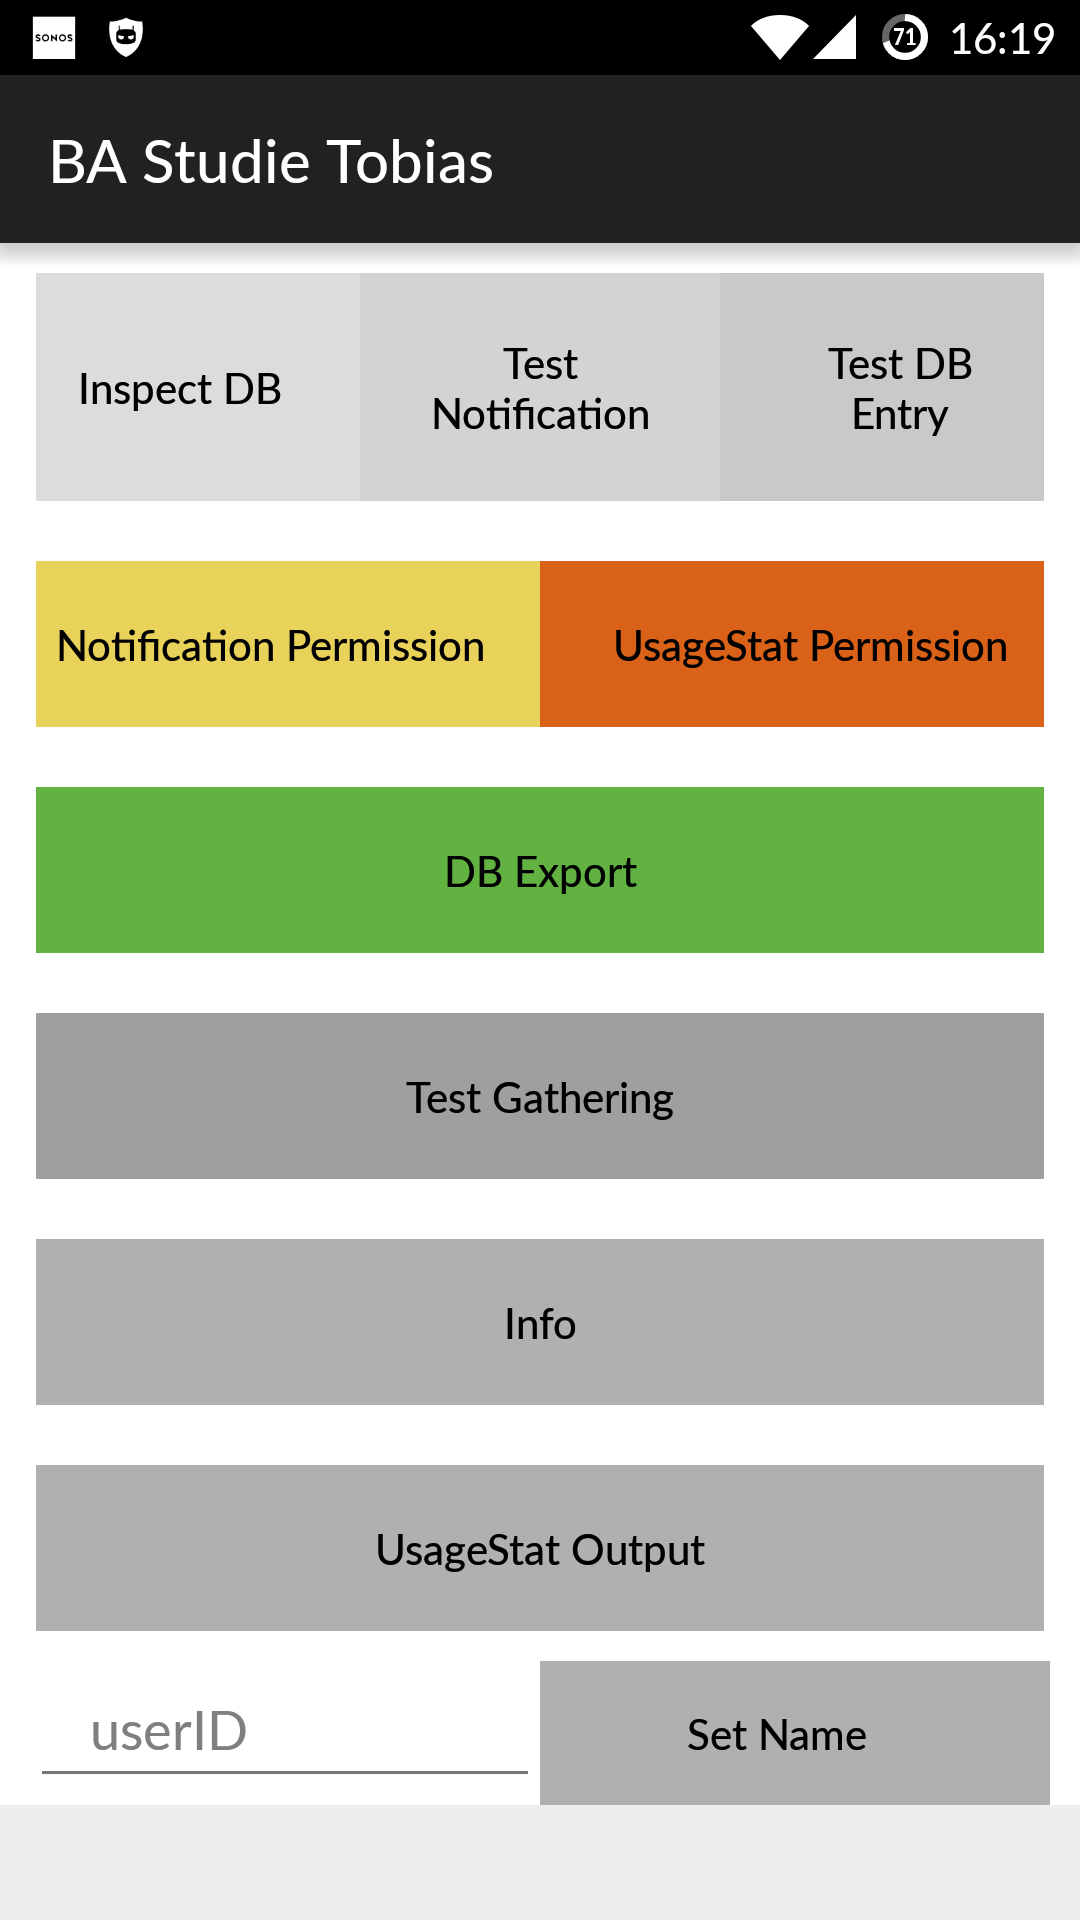
\includegraphics[width=0.4\textwidth]{images/screenshot1.png}
    \caption{User Interface der Applikation}
    \label{fig:uiscreen}
\end{figure}



Die erste Reihe an Buttons ermöglicht es - ohne Debuglogs lesen zu können - sicherzustellen, dass die Datenbank, in der die Applikation die Notifications aufzeichnet, nach dem Aufsetzen korrekt arbeitet.
Die Buttons in der zweiten Zeile ermöglichen das Erteilen der nichttrivialen Berechtigung, die die Applikation benötigt, durch die Nutzerin.
Der große grüne Knopf mit der Aufschrift "`DB Export"' wird von der Nutzerin benutzt, sobald die Studie abgeschlossen ist, um die gesammelten Daten zu exportieren.
Die Buttons in den Reihen vier und sechs sind wie schon die in der ersten Reihe dafür konzipiert, die korrekte Funktionsweise der Applikation zu gewährleisten.
Der mit dem Wort "`Info"' beschriftete Button in der fünften Zeile öffnet das Impressum der Applikation in einem AlertDialog.
Die siebte und unterste Reihe beinhaltet ein Textfeld und einen diesem zugehörigen "`Set Name"' Button.
Mit diesem kann die Nutzerin das von ihr gewählte und auf dem NEO-PI-R Fragebogen aufgeschriebene Pseudonym eintragen und mit dem Button bestätigen, um die Zuordnung von Fragenbogen zu Datensatz zu ermöglichen.
\section{Call und Message Logs}

Um mit der eigenen Applikation auf die vom Android Betriebssystem gesammelten Logs zu Anrufen und SMS zugreifen zu dürfen, müssen die Berechtigungen 
\textbf{android.permission.READ\_CALL\_LOG} und \textbf{android.permission.READ\_SMS} erteilt werden.
Diese können vom Programmierer in der AndroidManifest.xml Datei beantragt werden und können, da sie keine besonderen Permissions sind,
von der Nutzerin beim Installationsvorgang bestätigt werden.
\par
Mit dem Android \emph{contentResolver} kann nun eine Query durchgeführt werden, mit der die Applikation random read access auf die zurückgegebenen Daten erhält (siehe Code \ref{calllogquery}).
Über diese Daten kann nun iteriert werden und so die gewünschten Features extrahiert werden.
Mit jedem weiteren Eintrag wird die gesamte Anzahl und Gesamtdauer inkrementiert und die spezialisierten Aspekte von INCOMING, OUTGOING und MISSED werden per \emph{switch case} im Falle, dass das aktuelle Item ein ausgehender, ankommender oder verpasster Anruf ist, ebenfalls angepasst.
Die Zählung von einzigartigen Anrufpartnern geschieht hier über eine \emph{HashMap}, die eine AnruferID auf einen Integerwert mappt, der bei jedem Auftauchen dieser AnruferID um eins erhöht wird.
Nachdem so über alle Einträge iteriert wurde, werden die gesammelten Daten in einem \emph{CallData} Objekt gespeichert.
\par

Die Message Logs verhalten sich bis auf kleine Details identisch zu den Call Logs und können auf dieselbe Weise ausgewertet werden.
Ein Beispiel für ein solches Detail ist unter anderem, dass so etwas wie eine verpasste SMS nicht existiert und es nur SENT oder RECEIVED als Möglichkeiten gibt.
Die so gewonnen Daten werden im selben Objekt wie die Daten des Call Logs gespeichert und werden gemeinsam mit ihnen ausgegeben.

\begin{lstlisting}[frame=single, caption = Call Log Query, label=calllogquery] 
  getContentResolver().query(CallLog.Calls.CONTENT_URI, new String[] { CallLog.Calls.NUMBER, CallLog.Calls.DATE, CallLog.Calls.DURATION, CallLog.Calls.TYPE }, CallLog.Calls.DATE + ">?", new String[] { String.valueOf(resetDate.getTime())}, null);
\end{lstlisting}

\section{NotificationListenerService}

In der \emph{onCreate()} Methode der MainActivity wird der Service, wie in Code \ref{oncreateService} dargestellt, gestartet.
Entsprechend dem Wesen eines Service bei Android läuft dieser nun im Hintergrund weiter, selbst wenn die Applikation, die ihn gestartet hat, stirbt.
Sobald die Nutzerin die entsprechende Berechtigung erteilt, wird bei jeder eingehenden Notification die \emph{onNotificationPosted(StatusBarNotification sbn)} Methode mit der entsprechenden Notification als Argument aufgerufen.
Der NotificationService, der gestartet wurde, ist eine Subklasse des NotificationListenerService, in dem die  \emph{onNotificationPosted()} Methode so überladen wurde,
dass sie zusätzlich so ihrer normalen Funktion noch überprüft, ob die absendende Applikation eine der zu betrachtenden Applikationen ist und falls das der Fall ist, wie in Sektion \ref{ch:Implementierung:sec:Datenbank} beschrieben, einen neuen Eintrag in der Datenbank anlegt.
Dies geschieht, wie in Code \ref{validpackage} veranschaulicht, durch einen Zugriff auf das im Resourcen System abgelegte Array, das die relevanten Applikationen enthält. 
Das Android Resource System verwaltet alle Nicht-Code Assets der Applikation.
Das so erhaltene Array wird in ein HashSet übertragen, sodass mit dem Aufruf der \emph{contains()} Methode effizient überprüft werden kann, ob sich die absendende Applikation unter den relevanten befindet.


\begin{lstlisting}[frame=single, caption = startService(), label=oncreateService] 
  private Intent intentService;
  //...
  intentService = new Intent(this, NotificationService.class);
  startService(intentService);
\end{lstlisting}

\begin{lstlisting}[frame=single, caption = Package Überprüfung, label=validpackage] 
String[] temp = context.getResources().getStringArray(R.array.package_array);
        validPackages = new HashSet<>(Arrays.asList(temp));
\end{lstlisting}



\section{Datenbank}
\label{ch:Implementierung:sec:Datenbank}


Die Datenbank, in der die von der Applikation gelesenen Notifications gespeichert werden, ist eine SQLite Datenbank.
Dies ist naheliegend, da Android vollständigen Support für SQLite Datenbanken anbietet und wird standardmässig mit SQLite Version 3.4 ausgeliefert.
Die Erstellung der Datenbank wird von \emph{MySQLiteHelper}, einer Subklasse von SQLiteOpenHelper, in der \emph{onCreate()} Methode durchgeführt.
An diesem Ort wird auch das Layout der Datenbank ausgewählt:

\begin{lstlisting}[frame=single, caption = Datenbank Strings, label=databasestrings] 
    private static final String DATABASE_NAME = "notificationEntries.db";
    public static final String TABLE_NOTIFICATIONENTRIES = "notificationEntries"; 
    public static final String COLUMN_ID = "_id";
    public static final String COLUMN_NOTIFICATIONENTRY = "notificationEntry";
    public static final String COLUMN_TITLEHASHED = "titelHashed";
    public static final String COLUMN_TEXTLENGTH = "textLength";
    public static final String COLUMN_DATE = "date";
\end{lstlisting}

Hier werden die für das Anlegen der Datenbank relevanten Strings angelegt:
Der Name der Datenbank, der Name der Tabelle in der Datenbank und die Namen der Spalten werden daraufhin daraufhin genutzt, um den SQL Befehl zum Anlegen der Datenbank zusammenzusetzen.

\begin{lstlisting}[frame=single, caption = Datenbank Creation String, label=databasecreation] 
    private static final String DATABASE_CREATE = "create table "
            + TABLE_NOTIFICATIONENTRIES + "(" + COLUMN_ID
            + " integer primary key autoincrement, " + COLUMN_NOTIFICATIONENTRY + " text not null, " + COLUMN_TITLEHASHED + " text not null, " + COLUMN_TEXTLENGTH + " text not null," + COLUMN_DATE + " integer not null);";

\end{lstlisting}

Wie zu sehen wird hier eine Tabelle namens "`notificationEntries"' mit fünf Spalten angelegt.
In der ersten Spalte, der Spalte des primären Schlüssels, steht eine eindeutige ID, die mit weiteren hinzugefügten Zeilen selbstständig steigt.
In den restlichen Spalten stehen jeweils die relevanten Inhalte der Notifications, also absendende Applikation, der gehashte Titel und die Länge des Notificationtextes, als String und der Timestamp als Integer. 
Hier wird schon bei der Datenbankerstellung festgelegt, dass alle diese Werte nicht leer sein dürfen.

Die überschriebene \emph{onCreate()} Methode führt dann nur noch den hier festgelegten Tabellenerstellungsbefehl auf der Datenbank aus.

\begin{lstlisting}[frame=single, caption = onCreate Methode, label=databaseoncreate] 
  public void onCreate(SQLiteDatabase database) {
        database.execSQL(DATABASE_CREATE);
    } 
\end{lstlisting}

Neue Zeilen in der Tabelle können angelegt werden, indem ein \emph{ContentValues} Object gefüllt 
mit Tupeln aus den Spaltennamen und dem einzutragenden Wert angelegt wird und dieses dann mit der Methode \emph{insert} in die Datenbank eingesetzt wird.

\begin{lstlisting}[frame=single, caption = Einfügen in die Datenbank, label=databaseinsert] 
if (validPackages.contains(pack)) {
            ContentValues values = new ContentValues();
            values.put(MySQLiteHelper.COLUMN_NOTIFICATIONENTRY, pack);
            values.put(MySQLiteHelper.COLUMN_TITLEHASHED, hashedTitle);
            values.put(MySQLiteHelper.COLUMN_TEXTLENGTH, Integer.toString(textSize));
            values.put(MySQLiteHelper.COLUMN_DATE, System.currentTimeMillis());
            database.insert(MySQLiteHelper.TABLE_NOTIFICATIONENTRIES, null,
                    values);
            Log.d("db not", "Updated database");
        }
\end{lstlisting}

Zum Exportieren der Tabelle reicht es eine allgemeine Query auszuführen, die alle Zeilen zurück gibt, wie in Code 
\ref{databaseexport}.

\begin{lstlisting}[frame=single, caption = Einfügen in die Datenbank, label=databaseexport] 
  db.rawQuery("SELECT * FROM " + MySQLiteHelper.TABLE_NOTIFICATIONENTRIES,null); 
\end{lstlisting}

\section{UsageStats}

\section{Export}

Für den Export der gesammelten Daten wird im AndroidManifest.xml die Berechtigung \textbf{android.permission.WRITE\_EXTERNAL\_STORAGE}
benötigt. 
Diese ist keine außergewöhnliche Berechtigung und kann, wie die zum Zugang zu Call und Message Log, bei der Installation der Applikation beantragt werden.
\par
Die gesammelten Daten werden in drei Dateien in einem eigenen Ordner im \emph{ExternalStorageDirectory} des Smartphones gespeichert werden.
Sie werden als Comma Separated Values (csv) gespeichert.
Die Daten werden in die drei Dateien getrennt:

\begin{enumerate}
  \item Die Liste der erhaltenen Notifications
  \item Ergebnisse der Auswertung von Call Log und Message Log
  \item UsageStat Daten
\end{enumerate}
%nach Notification Daten, Anruf beziehungsweise SMS Daten und UsageStat Daten,

Dies geschieht, um das potenziell automatisierte Auswerten im Rahmen der Evaluation zu vereinfachen.
\par

Mit Hilfe von OpenCSV, einer einfachen Library zum Lesen und Schreiben von CSV Dateien \cite{opencsv},
wird zunächst die gesamte \\SQL Tabelle \textbf{TABLE\_NOTIFICATIONENTRIES} wie in Code \ref{databaseexport} angefragt und dann zeilenweise in eine Datei geschrieben.
Der Inhalt des callData Objekts wird als String entgegengenommen und nachdem es in einen StringArray gesplittet wurde, spaltenweise in die zweite Datei geschrieben.
In die dritte Datei werden die UsageStat Daten spaltenweise unter die zugehörigen Package Namen geschrieben.
\par
An alle Dateinamen wird die UserID der Nutzerin, aus der SharedPreference in der sie gespeichert wird, als Suffix angehängt um eine Zuordnung der Daten zu den Auswertungsergebnissen der Fragebögen zu ermöglichen.


\section{Geräte Tests}

Da nicht davon ausgegangen werden kann, dass alle Probandinnen über Smartphones mit vergleichbarer Leistung verfügen, muss die Applikation auch auf weniger leistungsstarken Geräten einwandfrei funktionieren.
Dies ist notwendig, um den komplikationsfreien Ablauf der Studie zu gewährleisten und mögliche Verluste von gesammelten Daten zu vermeiden.
Um dies zu sicher zu stellen wurde die Applikation auf zwei Geräten an verschiedenen Enden des Leistungsspektrums getestet:
Einerseits auf dem OnePlus One Smartphone, als primäres Entwicklungsgerät und Vertreter der leistungsstärkeren Smartphones und andererseits einem Motorola E (2nd Generation) als Vertreter für weniger leistungsstarke Smartphones eingesetzt wurde.
Wichtig waren hierbei die verschiedenen Spezifikationen:
Das OnePlus One ist ein Smartphone mit einem aktuellen 2.5GHz Quad-Core CPU, 3GB RAM und einem 5,5 Zoll 1920x1080 Pixel Display \cite{oneplusone}
während das Moto E (2nd Gen) als Vertreter der unteren Mittelklasse einen 1.2GHz Quad-Core CPU, 1GB RAM und ein 4,5 Zoll 540x960 Pixel Display hat \cite{motoe}.
Das OnePlus One verfügt mit seinem Akku mit 3100mAh über mehr Energiereserven als das Moto E, dessen Akku nur 2390mAh zur Verfügung stellt.
\par
Die Gerätetests waren erfolgreich, das Ausführen der Applikation beanspruchte auch auf dem signifikant schwächeren Gerät keine bemerkbaren Mengen an Ressourcen.



\section{Vorstudie}

Gegen Ende der Implementierung, nach dem groben Testen aller zu implementierenden Funktionalitäten, wurde eine kleine Vorstudie durchgeführt.
Dies geschah, um potenzielle Probleme bei der Hauptstudie frühzeitig zu entdecken und zu beheben, bevor sie negativen Einfluss auf die eigentliche Studie nehmen können.
Dazu wurde eine Vorabversion der entwickelten Applikation bei drei freiwilligen Testprobandinnen installiert.
Sie sollten über fünf Tage die Applikation im Hintergrund laufen lassen, sie auf Fehlverhalten untersuchen und die von der Applikation gesammelten Daten validieren.
Alle drei Freiwillige sind Informatikstudentinnen, zwischen 21 und 25 Jahren alt und regelmäßige Smartphone User, mit jeweils mehreren aktiv benutzten Kommunikationsapplikationen.
Die verwendeten Smartphones waren jeweils ein OnePlus One, ein OnePlus Two und ein Google Nexus 5.
\par
Jede der drei Freiwilligen bestätigte, dass die von der Applikation aufgezeichneten Daten korrekt waren.
Angemerkt wurde jedoch, dass das Userinterface relativ unübersichtlich sei und selbst mit Instruktionen, wie die Applikation aufzusetzen sei, dies, vor allem für weniger technologieaffine Probandinnen, relativ fehleranfällig sein könnte.
Eine der Probandinnen bemerkte, dass ein nicht zu vernachlässigender Teil ihrer Kommunikation, die über eine Applikation namens Signal laufe, nicht aufgezeichnet werde.
Auch die Wahl der Twitterclients wurde als nicht repräsentativ angemerkt:
Der Twitterclient "`Falcon Pro"' solle berücksichtigt werden.
Positiv wurde bemerkt, dass die Applikation nach dem Aufsetzen sehr ressourcensparend sei und keinerlei zusätzliche Interaktion von der Nutzerin benötigt.
Bei keiner der Freiwilligen kam es zu Abstürzen oder nicht vorgesehenem Verhalten. Auch nach mehrfachem Neustarten verrichtete die Applikation ihre Dienste wie beabsichtigt.
\par
Als Reaktion auf das Feedback aus der Vorstudie wurden folgende Dinge an der Applikation geändert:
Das Interface wurde überarbeitet und in einen übersichtlicheren, harmonischeren Zustand gebracht
In diesem Rahmen wurden für das Aufsetzen relevante Buttons durch farbliches Hervorheben kenntlich gemacht.
Die betrachteten Applikationen wurden um \emph{Falcon Pro}, einen weiteren Drittentwickler Twitterclient, und \emph{Signal}, einen allgemeine Kommunikationsapplikation mit starken Verschlüsselungs und Datenschutzfeatures, erweitert.
%Die Auswahl der zu betrachtenden Applikationen ist bereits so implementiert worden, dass man potenziell später ohne größere Probleme noch etwas hinzufügen oder entfernen kann.
Schon bei dem Entwurf der Applikation wurde darauf geachtet, das Hinzufügen und Entfernen von betrachteten Applicationen einfach zu gestalten.
Ansonsten wurde auf die Existenz des Android Features "`Privacy Guard"' hingewiesen, bei dem von der Testprobandin vermutet wurde, es könne mit dem Datensammeln interferieren.
Dies war jedoch nicht der Fall.
\par
Beim Versuch des Übertragens der Daten auf einen Computer kam ein Konflikt mit einem älteren Bug des Android Betriebssystems auf, der von Google im Oktober 2012 anerkannt wurde, jedoch bis heute nicht gefixt wurde
\cite{androidbug}.
Während dieser Bug der eigentlichen App keine Probleme bereitet, erspart Kenntnis dieses Umstandes potenziellen Testprobandinnen eventuelle Unannehmlichkeiten und damit verbundene Frustration beim Zurückführen der gesammelten Daten.


%%% Local Variables: 
%%% mode: latex
%%% TeX-master: "diplarb"
%%% End: 
